% Declare Document Class
\documentclass[a4paper,12pt,twoside,twocolumn,landscape]{book}

	% Latex Packages
\usepackage[T1]{fontenc}
\usepackage[utf8]{inputenc}
\usepackage{lmodern}
\usepackage{geometry}
\usepackage{listings}
\usepackage{color}
\usepackage[usenames,dvipsnames,svgnames]{xcolor}
\usepackage{graphicx}
\usepackage[numbers,square,sectionbib,comma,nonamebreak,elide]{natbib}
\usepackage{float}
\usepackage[english]{babel}
\usepackage{fancyhdr}
\usepackage{wrapfig}
\usepackage{array}
\usepackage{lipsum}
\usepackage{fancybox}
\usepackage{varwidth}
\usepackage{enumitem}
\usepackage{titlepic}
\usepackage[nottoc]{tocbibind}
\usepackage{url}
\usepackage[showisoZ]{datetime2}
\usepackage{transparent}
\usepackage{soul}
\usepackage{caption}
\usepackage{enumitem}
\usepackage{amssymb}
\usepackage{tikzsymbols} % http://ctan.math.utah.edu/ctan/tex-archive/graphics/pgf/contrib/tikzsymbols/tikzsymbols.pdf
\usepackage{textcomp}
\usepackage{parskip}
\usepackage{fourier}
\usepackage{array}
\usepackage{makecell}
\usepackage{inconsolata} 
\usepackage{blindtext}
\usepackage{expdlist} 
\usepackage{epigraph} % used to style quotes
\usepackage{titling} % makes available \thetitle \theauthor \thedate
\usepackage[toc,acronym,footnote,nomain]{glossaries} % Load the package with the acronym option
\usepackage{chngcntr}
\usepackage[unicode=false,
    colorlinks=true,
    linkcolor=darkgray,
    citecolor=darkgray,
    filecolor=darkgray,
    urlcolor=darkgray]{hyperref} % https://en.wikibooks.org/wiki/LaTeX/Hyperlinks


\catcode`\_=12


% styles list is available at
% https://www.sharelatex.com/learn/Natbib_bibliography_styles
\bibliographystyle{unsrtnat}


% Path where images are located relative
% to the file main.tex
\graphicspath{{img/}{figures/}}


% In which order to look after images in
% declared graphicspath{}'s
% 1. Low-quality JPG
% 2. Med-quality PNG
% 3. High-quality PDF
\DeclareGraphicsExtensions{.jpg,.png,.pdf}


\fancypagestyle{fancybook}{%
	\fancyhf{}%
	% Note the ## here. It's required because \fancypagestyle is making a macro (\ps@fancybook).
	% If we just wrote #1, TeX would think that it's the argument to \ps@fancybook, but
	% \ps@fancybook doesn't take any arguments, so TeX would complain with an error message.
	% You are not expected to understand this.
	\renewcommand*{\sectionmark}[1]{ \markright{\thesection\ ##1} }%
	\renewcommand*{\chaptermark}[1]{ \markboth{\chaptername\ \thechapter: ##1}{} }%
	% Increase the length of the header such that the folios 
	% (typography jargon for page numbers) move into the margin
	\fancyhfoffset[LE]{6mm}% slightly less than 0.25in
	\fancyhfoffset[RO]{6mm}%
	% Put some space and a vertical bar between the folio and the rest of the header
	\fancyhead[LE]{\color{GreenYellow}\thepage\hskip3mm\vrule\hskip3mm\leftmark}%
	\fancyhead[RO]{\color{GreenYellow}\rightmark\hskip3mm\vrule\hskip3mm\thepage}%
}
\pagestyle{fancybook}


% Use the roman numeric system for pagenumbers
\pagenumbering{roman}


% Usage: \pic[<pct-of-columnwidth>]{<path-to-file>}
\newcommand{\pic}[2][50]{
\begin{center}
    \transparent{0.4}
    \includegraphics[width=0.#1\columnwidth]{#2}
\end{center}
}

% Usage: \fig{<path-to-file>}{<label>}{<caption>}
\newcommand{\fig}[4]{
\begin{figure}[h!]
    \centering
    \includegraphics[width=0.95\columnwidth]{#1}
    \caption{#3}
    \label{fig:#2}
\end{figure}
}

% Usage: \svg{<path-to-file>}{<label>}{<caption>}
\newcommand{\svg}[3]{
    \begin{figure}[h]
        \centering
        \includesvg{#1}
        \caption{#3}
        \label{fig:#2}
    \end{figure}
}

\newcommand{\notice}[2]{%
    \shadowbox{%
        \begin{varwidth}{0.85\linewidth}
            \texttt{\textbf{#1}}\\
            #2
        \end{varwidth}
    }
}

\newcommand{\cliline}[2][]{\lstinline[columns=fixed,#1]{#2}}

\newcommand{\utccurrenttime}[0]{%
	\today%
	T%
	\DTMcurrenttime%
	\DTMfetchTZhour{now}%
	:%
	\DTMfetchTZminute{now}
} % Import user-defined commands


\definecolor{codegreen}{rgb}{0,0.6,0}
\definecolor{codegray}{rgb}{0.5,0.5,0.5}
\definecolor{codepurple}{rgb}{0.58,0,0.82}
\definecolor{backcolour}{rgb}{0.95,0.95,0.92}
 %user-defined colors


% https://tex.stackexchange.com/a/174553
\lstdefinestyle{mystyle}{
    language=cisco,
    backgroundcolor=\color{backcolour},
    commentstyle=\color{codegreen}\ttfamily,
    keywordstyle=\color{magenta},
    numberstyle=\tiny\color{codegray},
    stringstyle=\color{codepurple},
    basicstyle=\scriptsize\ttfamily,
    breakatwhitespace=false,
    breaklines=true,
    captionpos=b,
    keepspaces=true,
    numbers=left,
    showspaces=false,
    showstringspaces=false,
    showtabs=false,
    tabsize=4,
    abovecaptionskip=1em,
    aboveskip=1em,
    belowcaptionskip=1em,
    belowskip=3em,
    upquote=true,
    numbersep=8pt,
    rulecolor=\color{black},
}


\lstdefinestyle{plaintxt}{
    language=TeX,
    numbers=none,
    frame=trBL,
    frameround=fttt,
    backgroundcolor=\color{white},
    boxpos=c,
}


\lstdefinelanguage{cisco}{
    keywords={
        access-list,
        cdp,
        dhcp,
        end,
        hostname,
        interface,
        ip,
        line,
        lldp,
        login,
        network,
        no,
        ntp,
        router,
        show,
        shutdown,
        snmp-server,
        vlan,
        vrf
    },
    keywordstyle=\color{blue}\bfseries,
    ndkeywords={
        access-group,
        addr,
        address,
        aux,
        bgp,
        console,
        dhcp,
        eigrp,
        enable,
        fa,
        FastEthernet,
        gi,
        GigabitEthernet,
        group,
        host,
        ifindex,
        isis,
        ospf,
        ospfv3,
        pool,
        rip,
        run,
        view,
        vty
    },
    ndkeywordstyle=\color{darkgray}\bfseries,
    identifierstyle=\color{black},
    sensitive=false,
    comment=[l]{!},
    commentstyle=\color{purple}\ttfamily,
    stringstyle=\color{red}\ttfamily,
    caption=\lstname,
    tabsize=1,
    captionpos=t,
    showstringspaces=false,
    breaklines=true,
    breakatwhitespace=true,    
}


\geometry{a4paper,margin=1.5cm}
\setlength{\columnsep}{1.5cm} %space between columns
\setlength{\headheight}{15pt}
\setlength{\footnotesep}{0.5cm} %space between footnotes:
\setlength{\skip\footins}{2cm} %space between the text body and the footnotes
\setlist[itemize,1]{leftmargin=\dimexpr 26pt-.2cm}
\setlist[itemize,2]{leftmargin=\dimexpr 26pt-.3cm}
\lstset{style=mystyle} %apply lst styling


\renewcommand{\familydefault}{\sfdefault}


\DeclareCaptionFormat{myformat}{%
    % #1: label (e.g. "Table 1")
    % #2: separator (e.g. ": ")
    % #3: caption text
    \begin{varwidth}{\linewidth}%
        \centering
        #1#2#3%
    \end{varwidth}%
}
\captionsetup{format=myformat}% global activation


\newlist{todolist}{itemize}{2}
\setlist[todolist]{label=$\square$}
\usepackage{pifont}
\newcommand{\cmark}{\ding{51}}%
\newcommand{\xmark}{\ding{55}}%
\newcommand{\done}{\rlap{$\square$}{\raisebox{2pt}{\large\hspace{1pt}\cmark}}%
    \hspace{-2.5pt}}
\newcommand{\wontfix}{\rlap{$\square$}{\large\hspace{1pt}\xmark}}


\renewcommand\theadalign{cb}
\renewcommand\theadfont{\bfseries}
\renewcommand\theadgape{\Gape[4pt]}
\renewcommand\cellgape{\Gape[4pt]}

\def\tsq#1{\textquotesingle{#1}}
\def\bsq#1{%both single quotes
    \lq{#1}\rq}


\makeglossaries % Generate the glossary


\renewcommand*{\acronymname}{Abbreviations}


% Do not reset counter for footnotes at all
% through the document from start to finish.
% https://tex.stackexchange.com/a/10449
\counterwithout{footnote}{chapter}


% Do not reset counter for figures at all
% through the document from start to finish.
% https://tex.stackexchange.com/a/28334
\counterwithout{figure}{chapter}


% Set footnote numeration
% https://www.sharelatex.com/learn/Footnotes
% This command need to be run AFTER
% "\counterwithout{footnote}{chapter}" for the
% changes to be able to take effect.
\renewcommand{\thefootnote}{\arabic{footnote}}


\addtolength{\skip\footins}{2pt}    % vertical space between rule and main text


% https://tex.stackexchange.com/a/141975
\let\origfootnote\footnote % font size of footnotes; changes \footnotesize command only inside footnotes!
\renewcommand{\footnote}[1]{%
    \renewcommand\footnotesize\scriptsize % here there is scriptsize in footnotes (example)       
    \origfootnote{#1}}
 % Load structure cfg for document

%%%%%%%%%%%%%%%%%%%%%%%%%%%%%%%%%%%%%%%%%%%%%%%%%%%%%%
%                                                    %
% BEGIN DOCUMENT                                     %
%                                                    %
%%%%%%%%%%%%%%%%%%%%%%%%%%%%%%%%%%%%%%%%%%%%%%%%%%%%%%

\begin{document}

\DTMsavenow{now}

\title{Networking with switches and routers, automation and IPv4/6}
\def\thesubject{My Notes going along with learning Cisco Networking}
\def\theinstitution{ZBC}

\author{chhan11 <zbcchhan11 at zbc.dk>}
\def\thesupervisor{none}

\def\theversion{v0.4.0}
\date{{\footnotesize Last release \theversion\\%
    \texttt{\color{Gray}Generated \utccurrenttime}}}

\begin{titlepage}
    \centering
    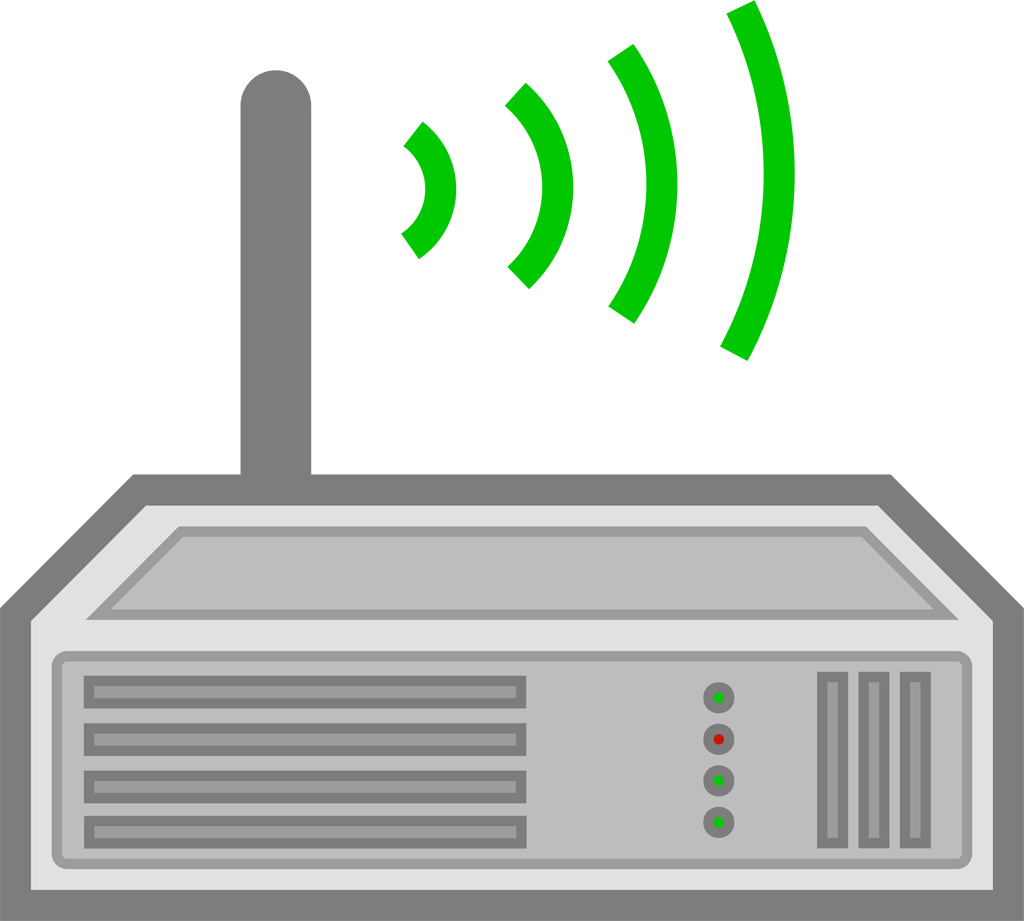
\includegraphics[width=0.15\textwidth]{router1}
    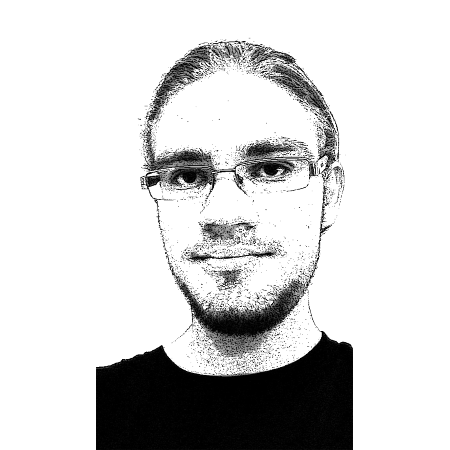
\includegraphics[width=0.15\textwidth]{profilepic/pic1}
    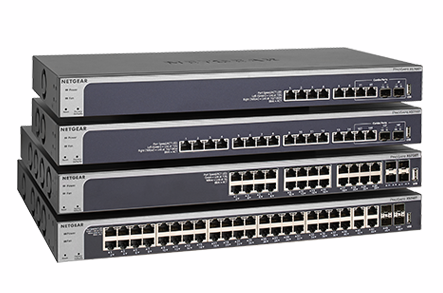
\includegraphics[width=0.15\textwidth]{switch1}
    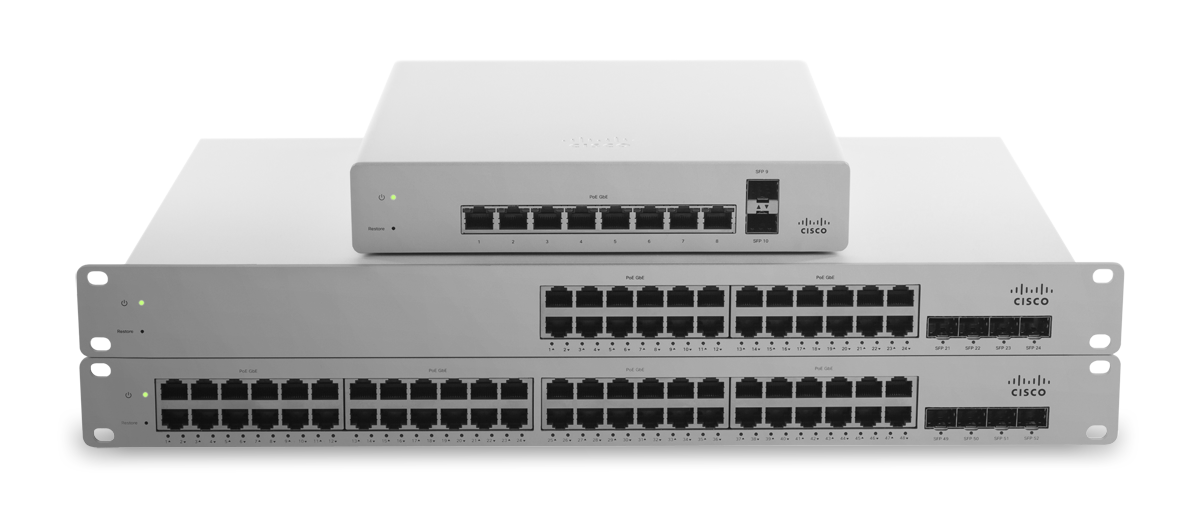
\includegraphics[width=0.15\textwidth]{switch2}
    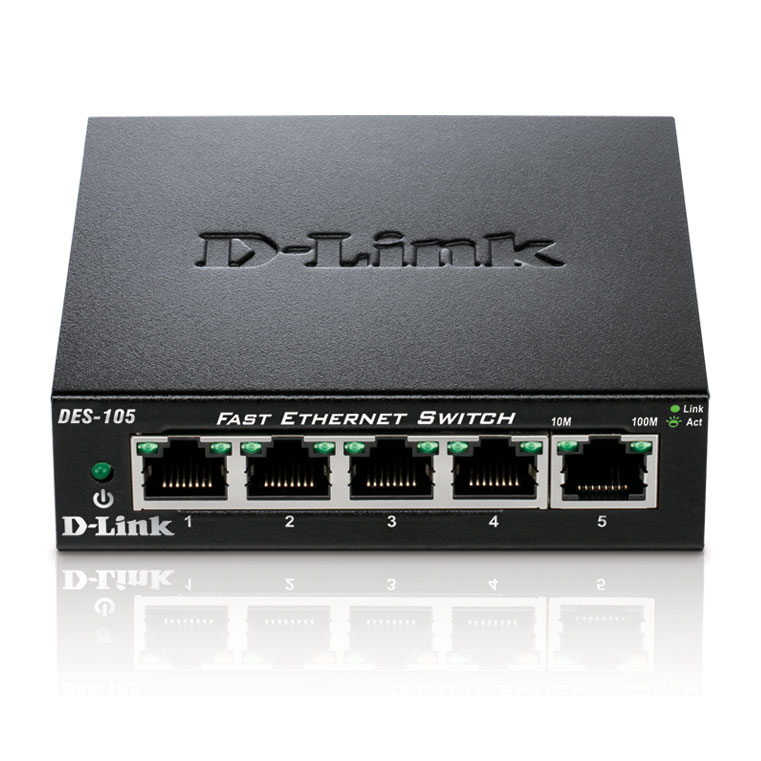
\includegraphics[width=0.15\textwidth]{switch3}
    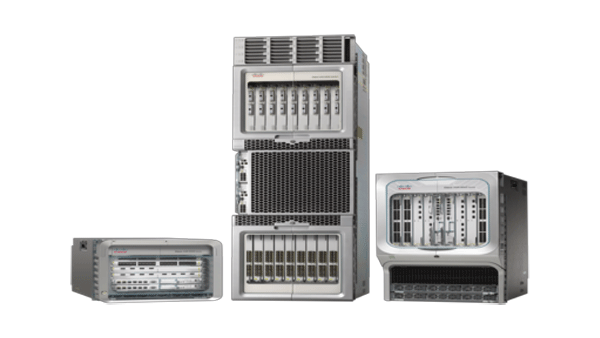
\includegraphics[width=0.15\textwidth]{router2}\par\vspace{1cm}
    {\scshape\LARGE \theinstitution\par}
    \vspace{1cm}
    {\scshape\Large \thetitle\par}
    \vspace{1.5cm}
    {\huge\bfseries \thesubject\par}
    \vspace{2cm}
    {\Large\itshape \theauthor\par}
    \vfill
    supervised by\par
    \thesupervisor
    
    \vfill
    
    % Bottom of the page
    {\large \thedate\par}
\end{titlepage}


\tableofcontents

% Only applied after generation of TOC
\setlength{\parskip}{0.35em} % Define length between paragrahps
\renewcommand{\baselinestretch}{1.15} % Define lineheight

%%%%%%%%%%%%%%%%%%%%%%%%%%%%%%%%%%%%%%%%%%%%%%%%%%%%%%
%                                                    %
% BEGIN chapters                                     %
%                                                    %
%%%%%%%%%%%%%%%%%%%%%%%%%%%%%%%%%%%%%%%%%%%%%%%%%%%%%%
	
% <!-- CONFIGURATION EXAMPLES -->

\chapter{Base Configuration}

\section{Cisco Lab}

\lstinputlisting[language=cisco]{code/base.cfg/base.cfg}
\lstinputlisting[language=cisco]{code/base.cfg/blockHSRPVRRPGLBP.cfg}
\lstinputlisting[language=cisco]{code/base.cfg/cdp.cfg}
\lstinputlisting[language=cisco]{code/base.cfg/clock.cfg}
\lstinputlisting[language=cisco]{code/base.cfg/dhcp.cfg}
\lstinputlisting[language=cisco]{code/base.cfg/hsrp.cfg}
\lstinputlisting[language=cisco]{code/base.cfg/interfaces.cfg}
\lstinputlisting[language=cisco]{code/base.cfg/lldp.cfg}
\lstinputlisting[language=cisco]{code/base.cfg/ntp.cfg}
\lstinputlisting[language=cisco]{code/base.cfg/ospf.cfg}
\lstinputlisting[language=cisco]{code/base.cfg/snmp.cfg}
\lstinputlisting[language=cisco]{code/base.cfg/ssh.cfg}
\lstinputlisting[language=cisco]{code/base.cfg/vty.cfg}


% <!-- LAYER 2 -->

\chapter{Layer 2}

\section{Switch Network}

\subsection{VTP}
\fig{vtp/implementing-vtp}{imp-vtp1}{VTP}

\subsubsection{VTP Modes}
The tree modes a VTP \textit{enabled} device can operate are
\begin{itemize}
    \item Transparent
    \item Server
    \item Client
\end{itemize}
Of course you can \textit{disable} VTP altogether.

Key things to be aware of \textit{before} enabling VTP in your environment is to make double sure of only having 1 VTP domain. \textbf{If} 2 or more VTP domains exists. Be triple sure to separate them! As to avoid having an VTP server DB overridden with data from another VTP domain.

The three VTP modes \textit{operates} as follow
\begin{itemize}
    \item Transparent
    \begin{itemize}
        \item Creates, modifies and deletes \textit{local} vlans only
        \item Forwards advertisements
        \item Does \textit{not} synchronizes vlan configurations.
    \end{itemize}
    \item Server
    \begin{itemize}
        \item Creates, modifies and deletes vlans
        \item Sends and forwards advertisements
        \item Synchronizes vlan configurations
    \end{itemize}
    \begin{itemize}
        \item Cannot create, modify or delete vlans
        \item Send and forwards advertisements
        \item Synchronizes vlan configurations
    \end{itemize}
\end{itemize}

\subsubsection{VTP Announcement}
VTP operates with announcements sent out in intervals. Summarized it amounts to
\begin{itemize}
    \item 1 \textit{summary} announcement per 5th minute from the server
    \item The summary announcement informs clients of the current revision
    \item An announcement is sent out \textit{on the spot} when a change has been made on the VTP server
\end{itemize}

Do remember it is \textbf{only} the VTP server which has the vlan configuration stored \textbf{on disk}. All device clients and transparent nodes do only store the vlans delegated by VTP in memory.

\subsubsection{Common Issues}
\begin{itemize}
    \item Different/Incompatible VTP versions
    \item Wrong password
    \item Incorrect mode name
    \item No server set (all devices configured in transparent/client/vtp disabled mode)
\end{itemize}

\subsubsection{VTP Versions}
\begin{itemize}
    \item Version 1
    \item Version 2
    \begin{itemize}
        \item Version-dependent	transparent	mode
        \item Consistencycheck
        \item Token ring support
        \item Unrecognized type-length-value support
    \end{itemize}
    \item Version 3 (not "yet" common)
    \begin{itemize}
        \item Extended VLAN support: Allow ranges are 1-1005,1018-2095. Not mentioned vlans ranges up to 4095 is still reserved.
        \item Domain name is not automatically learned.
        \item Better security.
        \item Better database propagation.
        \item MST now supported.
    \end{itemize}
\end{itemize}

\subsubsection{VTP Pruning}
The art of only allowing the vlan traffic to flow on \textit{necessary} links.

This means if there are no clients in a vlan on a device. Then no traffic for the inactive vlans is send down-/upstream on the link in question.
\fig{vtp/vtp-pruning}{vtpruning1}{VTP Pruning}

\subsubsection{Security}
It is \textbf{strongly} recommended to enable the security features supported in VTP.

\textbf{Password:} MD5 hashing, Case-sensitive, Length between 8 and 64 chars.

\notice{VTP Scaling}{
As the network grows and grows and grows and grows some more over long/short timespans.
You will \textbf{for certain} come to cross-rode, where you \textbf{must} consider to
go away from using VTP in the network. The problems of managing an elderly network and
wiping and re-introducing nodes in the network. You \textbf{will} face the issue of a
wiped vlan database from the VTP domain.
}

\subsubsection{Example configuration}
\lstinputlisting{code/vtp/example.cfg}

\subsection{Channel Bundling (aka. EtherChannel, PortChannel)}
Channel bundling is the "art" of using multiple physical links as one single logical link in when viewed from the perspective of the forwarding plane.

Technologies:
\begin{itemize}
    \item \textbf{PAgP:} The Cisco-only thingy
    \item \textbf{LACP:} The IEEE standard
    \item \textbf{Static:} Just forced on
\end{itemize}

\fig{channelbundling/network-without-channelbundling}{noethernetchannel}%
{No Channelbundling present}

Channel bundling of switch ports in the network may or may not be the best idea, in regards to the networks growth rate in terms of min. required bandwidth.

Channel bundling spreads out the in and egress flows based upon one of several methods configured on the switch:
\begin{itemize}
    \item Source to Destination MAC
    \item Source to Destination IP
\end{itemize}
Keep in mind this will by no means archive true load balancing. Where all links are equally used based upon number of flows \textit{or} in terms of used bandwidth.

\begin{table}[h]
    \centering
    \caption{Channel bundling mechanisms}
    \label{chbundmech1}
    \resizebox{\columnwidth}{!}{%
        \begin{tabular}{|l|l|l|}
            \hline
            Hash Input Code & Hash Input Detecision & Switch Model \\ \hline
            dst-ip          & Dest IP addr          & All models   \\ \hline
            dst-mac         & Dest MAC addr         & All models   \\ \hline
            src-dst-ip      & Src and dest IP addr  & All models   \\ \hline
            src-dst-mac     & Src and dest MAC addr & All models   \\ \hline
            src-ip          & Src IP addr           & All models   \\ \hline
            src-mac         & Src MAC addr          & All models   \\ \hline
            src-port        & Src port no           & 4500,6500    \\ \hline
            dst-port        & Dest port no          & 4500,6500    \\ \hline
            src-dst-port    & Src and dest port no  & 4500,6500    \\ \hline
        \end{tabular}%
    }
\end{table}

\fig{channelbundling/network-with-channelbundling}{withethernetchannel}%
{Channelbundling present}

\subsubsection{Protocol Properties}

\begin{itemize}
    \item LACP
    \begin{itemize}
        \item Active: Enabled
        \item Passive: Waits for LACP packets on the wire before enabled
    \end{itemize}
    \item PAgP
    \begin{itemize}
        \item Desirable: Enabled
        \item Auto: Waits for PAgP packets on the wire before enabled
    \end{itemize}
\end{itemize}

Some other \underline{required} settings to be (equal across all ports) aware of when configuring Channel bundling are
\begin{enumerate}
    \item Port speeds
    \item Duplex mode
    \item Configured vlan ranges
\end{enumerate}

\subsubsection{Example configuration}
\lstinputlisting{code/channelbundling/example.cfg}

\newpage

%%%%%%%%%%%%%%%%%%%%%%%%%%%%%%%%%%%%%%%%%%%%%%%%%%%%%%
%                                                    %
% SECTION BEGIN spanning tree protocol               %
%                                                    %
%%%%%%%%%%%%%%%%%%%%%%%%%%%%%%%%%%%%%%%%%%%%%%%%%%%%%%

\section{Spanning Tree}

Spanning Tree exists for the \textbf{sole} reason to save "your" network and all the broadcast storms an network engineer having a bad day can by mistake create!

STP comes from the above desire where redundancy was wanted but no protocol existed before STP to help in this regard.

\begin{table}[h]
    \centering
    \caption{Spanning Tree standrds}
    \label{stpstandards}
    \resizebox{\columnwidth}{!}{%
        \begin{tabular}{|l|l|l|l|l|}
            \hline
            \textbf{} & \textbf{Standard} & \textbf{Ressource Usage} & \multicolumn{2}{l|}{\textbf{Convergence}} \\ \hline
            CST       & 802.1D            & Low                      & Slow              & All vlans             \\ \hline
            PVST+     & Cisco             & High                     & Slow              & Per vlan              \\ \hline
            RSTP      & 802.1w            & So-so (Med.)             & Fast              & All vlans             \\ \hline
            RPVST+    & Cisco             & On-the-double (V.High)   & Fast              & Per vlan              \\ \hline
            MST       & 802.1s            & Med. - High              & Fast              & Vlan list             \\ \hline
        \end{tabular}%
    }
\end{table}

\subsection{Port Roles}

When a switch is enabled for Spanning Tree. One of the following roles will have been assumed by any port on the switch in question.

\begin{itemize}
    \item \textbf{Root port:} Only 1 port on any switch (non-counting the root bridge!). Is always the port with the lowest metric (aka. best path) to the root bridge.
    \begin{itemize}
        \item The upstream/-link port closest to the root bridge on all switches apart from the root bridge.
    \end{itemize}
    \item \textbf{Designated port:} A designated port is the port on any segment closest to the root bridge and forwarding traffic.
    \begin{itemize}
        \item The port on any switch in downstream direction closet to the root bridge.
    \end{itemize}
    \item \textbf{\textit{Non}-designated port:} Put in blocking mode and not currently forwarding traffic.
    \begin{itemize}
        \item All switch ports which did not get elected as the root or designated port.
    \end{itemize}
    \item \textbf{Disabled port:} The port has been one-way-or-another shut down.
\end{itemize}

\subsubsection{specific port roles}
\begin{itemize}
    \item \textbf{Alternative port} is an active port in network with an alternative path to the root bridge. A port in alternative mode will remain active but \textit{discards} all traffic until the the current designated path fails.
    \item \textbf{Backup port} is running in active mode and \textit{discards} all traffic it recieves until the current designated port on the segment the backup port is connected to, fails.
\end{itemize}

Election of ports goes in order of the following values (low is best): 1) root bridge id, 2) lowest path cost to root bridge, 3) sender bridge id, 4) sender port bridge id

%%%%%%%%%%%%%%%%%%%%%%%%%%%%%%%%%%%%%%%%%%%%%%%%%%%%%%
%                                                    %
% SECTION BEGIN standards                            %
%                                                    %
%%%%%%%%%%%%%%%%%%%%%%%%%%%%%%%%%%%%%%%%%%%%%%%%%%%%%%

\subsection{Standards}

\begin{itemize}
    \item STP {\scriptsize Spanning Tree Protocol}
    \begin{itemize}
        \item IEEE 802.1D
        \item Was created in a time where bridged networks was the norm.
        \item Supports a single vlan/lan.
    \end{itemize}
    \item CST {\scriptsize Common Spanning Tree}
    \begin{itemize}
        \item An evolution of stp
        \item Cst still only supports one STP instance.
        \item But CST do thou in contrast to STP support \textit{multiple} vlans.
    \end{itemize}
    \item PVST {\scriptsize Per Vlan Spanning Tree}
    \begin{itemize}
        \item Now obsolute and succeded by PVST+
    \end{itemize}
    \item PVST+ {\scriptsize Per Vlan Spanning Tree Plus}
    \begin{itemize}
        \item Runs an instance of STP per vlan.
        \item Can guarante better utilization of available network bandwidth.
        \item Root bridge and port priorities can be configured per vlan.
        \item Uses the term alternate for nondesignated port.
    \end{itemize}
    \item RSTP {\scriptsize Rapid Spanning Tree Protocol}
    \begin{itemize}
        \item IEEE 802.1w
        \item A future development of the original 802.1D standard meant to provide faster convergance. As the original STP standard wasn't actually that fast.
    \end{itemize}
    \item RPVST+ {\scriptsize Rapid Per Vlan Spanning Tree Plus}
    \begin{itemize}
        \item A cisco implementation of RSTP based upon pvst+.
    \end{itemize}
    \item MST {\scriptsize Multiple Spanning Tree}
    \begin{itemize}
        \item Originally a cisco developed protocol. MST has since been developed as an IEEE standard.
        \item MST can as CST map multiple vlans to a single STP instance.
        \item MST \textit{differently} than CST supports multiple STP instances.
        \item Fx. Instance 1: Vlan 1-99, Instane 2: Vlan 100-199.
    \end{itemize}
\end{itemize}

\subsection{Features}

\subsubsection{BPDU}
\textbf{B}ridge \textbf{P}rotocol \textbf{D}ata \textbf{U}nits is on cisco equipment sent out every 2 seconds and generally catogorizes into 2 categories:
\begin{itemize}
    \item \textit{Configuration} BPDU used for STP calculations and
    \item \textit{Topology change notifications} BPDUs used to notify other network nodes of a change in the network.
\end{itemize}

Any network node with switchports and STP + BPDU enabled sends out BPDU packets with the ports mac as the src address. The destination mac is is designated STP multicast addr 01:80:C2:00:00:00.

\subsubsection{Root Bridge}
Using a \textbf{R}oot \textbf{B}rigde as the reference point for the STP instance and calculation of root/designated/non-designated ports.\\This election process uses a pre-configured bridge priority (ranges from $0$ to $2^{16}$) (defaults to $2^{15}$). If a tie in priority is found the switch in possession of the lowest mac address wins the root bridge election.


\subsubsection{Port Cost}

\begin{table}[h]
    \centering
    \caption{Default port cost in spanning tree}
    \label{stpportcost}{!}{%
        \begin{tabular}{|l|l|}
            \hline
            \textbf{Link} & \textbf{Default Cost} \\ \hline
            10 Gbps       & 1                     \\ \hline
            1 Gbps        & 4                     \\ \hline
            100 Mbps      & 19                    \\ \hline
            10 Mbps       & 100                   \\ \hline
        \end{tabular}%
    }
\end{table}

\fig{spanningtree/portroles}{stpportroles}{Port Election}

\textit{\textbf{NB:} beware that when working with bundled links (aka. ether-/port-channel). Then the link cost will be calculated based upon the summarized bandwidth accross all links.}

\fig{spanningtree/portstates}{stpportstates}{Port States}

\section{Rapid Spanning Tree Protocol}

\fig{rstp/portroles}{rstpportroles}{Port Roles}

\fig{rstp/portlinktypes}{rstpportlinktypes}{Port link types}

Things to be aware of regarding RSTP port roles
\begin{itemize}
    \item \textbf{Shared} port state will only ever be present on segments where a hub is present.
    \item \textbf{Point-2-Point} port is connected to a single switch on the other end.
    \item \textbf{Edge} port roles is only ever connected to end devices. Status as Edge port is lost if a BPDU is ever recieved.
\end{itemize}

%%%%%%%%%%%%%%%%%%%%%%%%%%%%%%%%%%%%%%%%%%%%%%%%%%%%%%
%                                                    %
% SECTION BEGIN port roles                           %
%                                                    %
%%%%%%%%%%%%%%%%%%%%%%%%%%%%%%%%%%%%%%%%%%%%%%%%%%%%%%

\section{Port roles}

\subsection{Fast port roles}
Cisco did on their part early on enhance the original spanning tree standard with some proprietary portroles that can (on cisco switch equipment) skip steps in the port role election process. And configure a STP switchport to a specific behavior as described below:

\begin{itemize}
    \item PortFast
    \begin{itemize}
        \item Configures access port to transition directly to forwarding state.
        \item Improve convergence times of non-RSTP.
        \item Port does no forwan TCN\footnote{\textbf{Needs finding out what TCN is.}} BPDUs either.
        \item PortFast can be enabled either A) per port \textit{or} B) globally for all ports in access mode.
        \begin{enumerate}
            \item Per port: {\footnotesize Accesss port}\\\cliline{cisco-switch(config-if)# spanning-tree portfast}
            \item Per port: {\footnotesize Trunk port}\\\cliline{cisco-switch(config-if)# spanning-tree portfast trunk}
            \item Globally:\\\cliline{cisco-switch(config)# spanning-tree portfast default}
        \end{enumerate}
    \end{itemize}
    \item UplinkFast
    \begin{itemize}
        \item Enables fast uplink failover on access switch.
        \item Improve convergence times of non-RSTP.
        \item Enabled only with non-RSTP
        \item Integrated into Cisco's RSTP implementaion and enabled by defaut.
        \item Cisco proprietary
        \item Only works if switch has blocked ports
        \item Designed with switches in access layer as deployment target.
        \item Enabled for the entire switch. Cannot be enabled pr. vlan.
        \item \cliline{cisco-switch(config)# spanning-tree uplinkfast} enables the feature.
    \end{itemize}
    \item BackboneFast
    \begin{itemize}
        \item Enables fast convergence in distribution or core layer when STP change occurs.
        \item Improve convergence times of non-RSTP.
        \item Enabled only with non-RSTP
        \item Integrated into Cisco's RSTP implementaion and enabled by default.
        \item Disabled by default
        \item \cliline{cisco-switch(config)# spanning-tree backbonefast} enables the feature.
        \item \textit{Scenario:} If switch needs searching new path root bridge. BackboneFast shortens process.
        \begin{enumerate}
            \item Switch will search for alternative path to root.
            \item If BPDU recieved on blocked port. Port considered alternative path path to root.
            \item If alternate path identified. RQL{\footnotesize \textbf{R}equest \textbf{L}ink \textbf{B}locking} packets are out for identify either A) an alternative path to the root bridge \textit{or} B) an up-/downstream switch with a path to the root bridge.
        \end{enumerate}
    \end{itemize}
\end{itemize}

\subsection{Loop Prevention}

\begin{itemize}
    \item BPDU Guard
    \begin{itemize}
        \item Disables the PortFast-enabled port if a BPDU is received. The port goes into mode \texttt{err-disable}.
        \item Enable per port:\\\cliline{cisco-switch(config-if)# spanning-tree bpduguard enable}
        \item Enable globally for portfast enabled ports:\\\cliline{cisco-switch(config)# spanning-tree portfast bpduguard default}
    \end{itemize}
    \item BPDU Filter
    \begin{itemize}
        \item Suppresses BPDUs on ports
        \item Behaves differently depending if enabled
        \item A) globally \textit{or}
        \begin{enumerate}
            \item Affects all active portfast enabled ports, which \underline{don't} have a BPDU port configuration.
            \item If BPDU recieved on port, portfast and BPDU filter is disabled.
            \item Sends \textbf{10} BPDUs on startup. If BPDU recieved in this timeframe \textit{same consequence as above} happens to the port.
            \item \cliline{cisco-switch(config-if)# spanning-tree bpdufilter enable}
        \end{enumerate}
        \item B) per-port:
        \begin{enumerate}
            \item Port ignores all recieved BPDUs.
            \item Port sends no BPDUs.
            \item \cliline{cisco-switch(config-if)# spanning-tree bpdufilter enable}
        \end{enumerate}
        \item Beware to \underline{only} enable BPDU filter on ports connected to end hosts. Consequence if not followed \underline{can} result in creating bridging loops.
        \item Beware to \underline{only enable either} BPDU guard \textbf{\textit{or}} filter. \footnote{Cisco recommendation}
    \end{itemize}
    \item Root Guard
    \begin{itemize}
        \item \st{Prevents external switches from becoming roots}
        \item If enabled, prevents any ports from becoming a root-port. Ports will remain as designated ports \textit{effectivily} preventing the switch becoming the root bridge.
        \item This, too, behaves in s similiar manner as BPDU guard, putting the port in \texttt{err-disable} mode when a BPDU packet is recieved on the port.
        \item Enabled per-port with\\\cliline{cisco-switch(config-if)# spanning-tree guard root}
    \end{itemize}
    \item Loop Guard
    \begin{itemize}
        \item Prevents an alternate port from becoming the designated port if no BPDUs are received
        \begin{enumerate}
            \item Normally when cisco swicthes stop recieving BPDUs ingress in a port. The port will go to listeting, learning, forwarding state equaling a loop.
            \item With Loop guard enabled the will go to \texttt{loop-inconsistent} blocking state instead.
        \end{enumerate}
        \item Enabled per-port\\\cliline{cisco-switch(config-if)# spanning-tree guard loop}
        \item Enabled globally\\\cliline{cisco-switch(config)# spanning-tree loopguard default} {\small only on p2p links}
        \item Works on per-vlan basis when PVSTP is used.
        \item On ether-channel links with uni-directional link failures, loop guard will put put the whole ether-channel into loop-inconsistent state.
    \end{itemize}
    \item \textbf{Beware} root and loop guard is mutually exclusive
    \begin{itemize}
        \item Root guard works on designated ports and does not allow the ports to become \textit{non}-designated ports, where
        \item Loop guard works on \textit{non}-designated ports and does not allow the ports to become designated ports {\footnotesize though expiration of times}.
    \end{itemize}
\end{itemize}

\subsection{Link}

\begin{itemize}
    \item Unidirectional Link Detection (UDLD)
    \begin{itemize}
        \item Cisco proprietary feature.
        \item By default only enables on fiber optic links.
        \item Works by sending packes every 15 seconds (default timer). If not packet is recieved back, the port can either log (default) a messaage or actively try to re-establish the link (aggresive). 1 packet/second for 8 sec. is send. If non is returned the port will go to \texttt{err-disable} state.
        \item \cliline{cisco-switch(config)\# udld \{enable | aggresive\}}
        \item On ether-channel links with uni-directional link failures, udld will disable individual failed links.
        \item For the best protection. Aggresive mode is recommended.
        \item It is recommended to turn on udld in global conf mode.
    \end{itemize}
    \item FlexLinks
    \begin{itemize}
        \item Cisco proprietary feature.
        \item An alternate solution to running STP in the environment.
        \begin{itemize}
            \item STP is auto-disabled on interfaces running FlexLinks.
            \item Configured with 2 physical links with and active/backup configuration.
            \item Enables convergence time of less than 50 milliseconds.
        \end{itemize}
        \item FlexLinks is good alternative to running STP in an environment with customers who you do \textit{not} want to run STP with. Fx. Service Provider/Enterprise/Datacenter environment.
        \item Preemtion for FlexLinks is \textit{not} enabled-by-default.
        \begin{enumerate}
            \item Detects link failure.
            \item Moves any dynamic unicast MAC addresses learned on primary link to standby link.
            \item Moves standby link to forwarding state.
            \item Transmits dummy multicast packets over new active interface. {\small Dummy multicast packet format is as follows: \textbf{destination:} 01:00:0c:cd:cd:cd, \textbf{source:} MAC address of the hosts or ports on the newly active FlexLinks port}
        \end{enumerate}
        \item {\small \textbf{Note:}} Configuring FlexLinks outside of access layer switches can be very complex!
        \item Enabled FlexLinks on an interface: \\
            \cliline{cisco-switch(config)# interface fa0/1} \\
            \cliline{cisco-switch(config-if)# switchport backup interface fa0/2}
        \item \textbf{What} FlexLinks can be:
        \begin{enumerate}
            \item A physical port
            \item A Bundled link {\footnotesize (aka. ether-channel)}
            \item 1 FlexLink per physical/logical port
            \item Link speeds need not be the same
        \end{enumerate}
    \end{itemize}
\end{itemize}

\begin{table}[h]
    \centering
    \caption{UDLD|Loopguard compared}
    \label{udldloopguard}
    \resizebox{\columnwidth}{!}{%
        \begin{tabular}{|l|l|l|}
            \hline
            \thead{Functionality} & \thead{Loop guard} & \thead{UDLD} \\ \hline
            Action granularity & Per vlan & Per port \\ \hline
            \makecell{Protection against STP\\failures caused by uni-directional\\ links} & \makecell{Yes, when enabled on all\\potential non-designated ports\\in redundant topology} & \makecell{Yes, when enabled on all\\links in redundant topology} \\ \hline
            \makecell{Protection against STP\\failures caused by problem in\\software resulting in designated\\switch not sending BPDUs} & Yes & No \\ \hline
            Protection against mis-wiring & No & Yes \\ \hline
        \end{tabular}%
    }
\end{table}

\fig{spanningtree/stpbestpractice}{stpbestpractice}{STP best practice}

\section{Multiple Spanning Tree}

\begin{itemize}
    \item \itemtitle{Known limitations}{Regarding the cisco world of things}
    \begin{enumerate}
        \item A maximum of 16 instances is supported. {\footnotesize From 0 to 15.}
    \end{enumerate}
    \item \textbf{Beware} that instance 0 is the \textit{I}nternal \textit{S}panning \textit{T}ree. And therefore cannot be configured for user-mapped Vlans.
    \item Aggregates the configured vlans into groups/instances/processes. This in turn provides lower resource utilization on switches. \dWinkey
    \item Backwards compatible with 802.1D STP/802.1w/RSTP and Cisco PVST+.
    \item Converges faster than PVRST+.
    \item \itemtitle{Challenges}{Arises because of older hardware and the architecture of the protocol}
    \begin{enumerate}
        \item Operability with older/legacy hardware/equipment is not always possible.
        \item \textit{Of course} it is more complex compared to standard STP (older) protocols. {\footnotesize Staff may require teachings of the way of the protocol.}
    \end{enumerate}
\end{itemize}

\begin{table}[h]
    \centering
    \caption{MST Attributes}
    \label{mstattr}
    \resizebox{\columnwidth}{!}{%
        \begin{tabular}{|l|l|}
            \hline
            \thead{Data} & \thead{What ?} \\ \hline
            32 bytes & alphanumeric configuration name \\ \hline
            2 bytes & configuration revision number \\ \hline
            Table of 4096 elements & \makecell{associates each of the potential\\4096 VLANs with an instance} \\ \hline
        \end{tabular}%
    }
\end{table}

\subsection{MST Regions}

It is the network admins job to propagate an even configuration to all switches in a single region by using CLI or SNMP. Currently IOS does not support any other options to do the job.

\begin{itemize}
    \item \itemtitle{Boundaries}{MST differs between regions by}
    \begin{enumerate}
        \item sending a digest computer from the Vlan-to-instance mapping table of the switch sending the digest.
        \item the characteristics of the MST protocol for that single switch.
    \end{enumerate}
    \item if computed digest and MST characteristics between switches is \textit{found matching}, the switches considers themselves part of the same MST region.
    \item \textbf{Beware} that unlike VTP, MST does not automatically increase the configuration revision number. This \textit{has to be done} manually.
\end{itemize}

\fig{spanningtree/mstregions}{mstregions}{MST Regions all Vlans running mappen to the default instance 0.}

\fig{spanningtree/mstregions2}{mstregions2}{MST Regions vlans mapped to different instances.}

\begin{lstlisting}[language=TeX,numbers=none,frame=trBL,frameround=fttt,backgroundcolor=\color{white}]
+----------+-----------+---------+
| Bridge   | Extended  | MAC     |
| priority | system ID | Address |
+----------+-----------+---------+
\end{lstlisting}

% <!-- INTERVLAN -->

\chapter{L2 to L3}

\section{Vlan-to-vlan routing}

% <!-- DHCP -->

\chapter{DHCP}

\section{Process}

\fig{dhcp/dhcpdiscoverprocess}{dhcpdiscoverprocess}{DHCP Discover Process}

\subsection{DHCP Messages}

\begin{itemize}
    \item \textbf{DHCPDECLINE:} Message sent from the client to the server that the address is already in use.
    \item \textbf{DHCPNAK:} The server sends a refusal to the client for request for configuration.
    \item \textbf{DHCPRELEASE:} Client tells a server that it is giving up a lease.
    \item \textbf{DHCPINFORM:} A client already has an IP address but is requesting other configuration parameters that the DHCP server is configured to deliver such as DNS address.
\end{itemize}

\section{Example configuration}

\subsection{Cisco}

\begin{txt}
ip dhcp excluded-address 192.168.0.254
!
ip dhcp pool LAN-1-POOL-DHCP
 network 192.168.0.0 255.255.255.0
 default-router 192.168.0.254
 lease 2 ! set in days
\end{txt}

When configuring a Layer 3 interface as a relay port for DHCP request for a subnet. Set the ip helper command on the interface with one \textit{or} more ip addresses.

\begin{txt}
interface GigabitEthernet 0/3
 ip helper-address 192.168.220.220
 ip helper-address 192.168.222.222
\end{txt}


% <!-- VRRP, GLBP, HSRP -->

\chapter{1st hop failure/failover/redundancy}

\section{VRRP}

\section{GLBP}

\section{HSRP}

% <!-- ACCOUNTING AND LOGINS, RADIUS, TACACS+ -->

\chapter{Triple A\tsq{s}}

\myquote{}{Remember to log the details, too.}

\xkcd{latitude}{Remember logging when necessary}

\newpage

\begin{itemize}
    \item \textbf{Authentication:}
    \begin{enumerate}
        \item Identify the user,
        \item Validate the user,
        \item Allow/Disallow user based upon credentials.
    \end{enumerate}
    \item \textbf{Authorization:}
    \begin{enumerate}
        \item Have defined levels of allowed operations/tasks divided into groups,
        \item Validate user-to-groups relations,
        \item Allow/Disallow user actions.
        \item On network gear the Allow/Disallowed actions can be stored on either the central AAA server or locally\footnote{May not apply to all network gear} in the network node.
    \end{enumerate}
    \item \textbf{Accounting:}
    \begin{enumerate}
        \item Network nodes collect user and session information from start to end when connecting to a node,
        \item All information is transferred back to AAA server,
        \item Transferred info can be leveraged for several purposes. Typically logged info is:
        \begin{itemize}
            \item session duration,
            \item user commands,
            \item disallowed commands
        \end{itemize}
    \end{enumerate}
\end{itemize}

\section{RADIUS}

\section{TACACS+}


% <!-- NTP -->

\chapter{Network Time Protocol}

\section{The old NTP from \tsq{85}}

\section{Secure NTP}

% <!-- NETWORK MANAGEMENT -->

\chapter{Managemnt}

\section{Network management}

\subsection{Routers}

\subsection{Switches}

\subsection{Firewall}

\section{Out-of-band management}

\subsection{Console server}

% <!-- LAYER 3 STUFF -->

\chapter{Protocols Layer 3}

\section{Routed Network}

\section{OSPF}
\section{IS-IS}
\section{EIGRP}
\section{RIP}
\section{Static}
\section{BGP}


% <!-- DESCRIBE THE INTERNET -->

\chapter{The Internet {\footnotesize "Post cold-war modern times"}}

\section{Service Providers}

\section{IXP}

\section{MPLS}

\section{BGP}

\section{eVPN}

%%%%%%%%%%%%%%%%%%%%%%%%%%%%%%%%%%%%%%%%%%%%%%%%%%%%%%
%                                                    %
% BEGIN list of figures                              %
%                                                    %
%%%%%%%%%%%%%%%%%%%%%%%%%%%%%%%%%%%%%%%%%%%%%%%%%%%%%%

\renewcommand{\listfigurename}{List of {\footnotesize hidden} Figures}
\listoffigures

%%%%%%%%%%%%%%%%%%%%%%%%%%%%%%%%%%%%%%%%%%%%%%%%%%%%%%
%                                                    %
% BEGIN list of tables                               %
%                                                    %
%%%%%%%%%%%%%%%%%%%%%%%%%%%%%%%%%%%%%%%%%%%%%%%%%%%%%%

\renewcommand{\listtablename}{Tables {\footnotesize hidding} on the pages}
\listoftables

%%%%%%%%%%%%%%%%%%%%%%%%%%%%%%%%%%%%%%%%%%%%%%%%%%%%%%
%                                                    %
% BEGIN references                                   %
%                                                    %
%%%%%%%%%%%%%%%%%%%%%%%%%%%%%%%%%%%%%%%%%%%%%%%%%%%%%%

\bibliography{references}

%%%%%%%%%%%%%%%%%%%%%%%%%%%%%%%%%%%%%%%%%%%%%%%%%%%%%%
%                                                    %
% END DOCUMENT                                       %
%                                                    %
%%%%%%%%%%%%%%%%%%%%%%%%%%%%%%%%%%%%%%%%%%%%%%%%%%%%%%

\end{document}
